% Resultados
\chapter{Implementación} \label{sect:impresultados}

    En este proyecto de grado, se implementaron cinco metaheurísticas (los algoritmos
\emph{genético}\cite{DoGeGr2007}, \emph{de abeja}\cite{BEE_0} y \emph{de hormiga}
\cite{OuBa2007}, la \emph{evolución diferencial}\cite{SwAjAm2008} y el \emph{optimizador
de enjambre de partículas}\cite{PSO_0}) y el algoritmo determinista \emph{K-means}
\cite{GePo2010} para la resolución del problema de \emph{data clustering}.
\begin{comment}y se
realizó un estudio comparativo de sus desempeños. El objetivo principal es
identificar las metaheurísticas que mejor resuelvan el problema de clustering de
datos numéricos, es decir, que sus soluciones finales tengan la mejor calidad.
\end{comment}

\section{Lenguaje usado} \label{sec:lusado}
    Los algoritmos fueron implementados en C++. Se eligió este lenguaje debido
a que compila a código de máquina, permite el eficiente manejo de
recursos del sistema y es orientado a objetos lo cual facilita una buena
abstracción de los problemas por medio del uso de clases. Además, cuenta con
muchas utilerías implementadas, lo que ayudó al ahorro del tiempo de implementación
del proyecto.

El diagrama de clases es el siguiente:

\begin{figure}[htb]
\centering
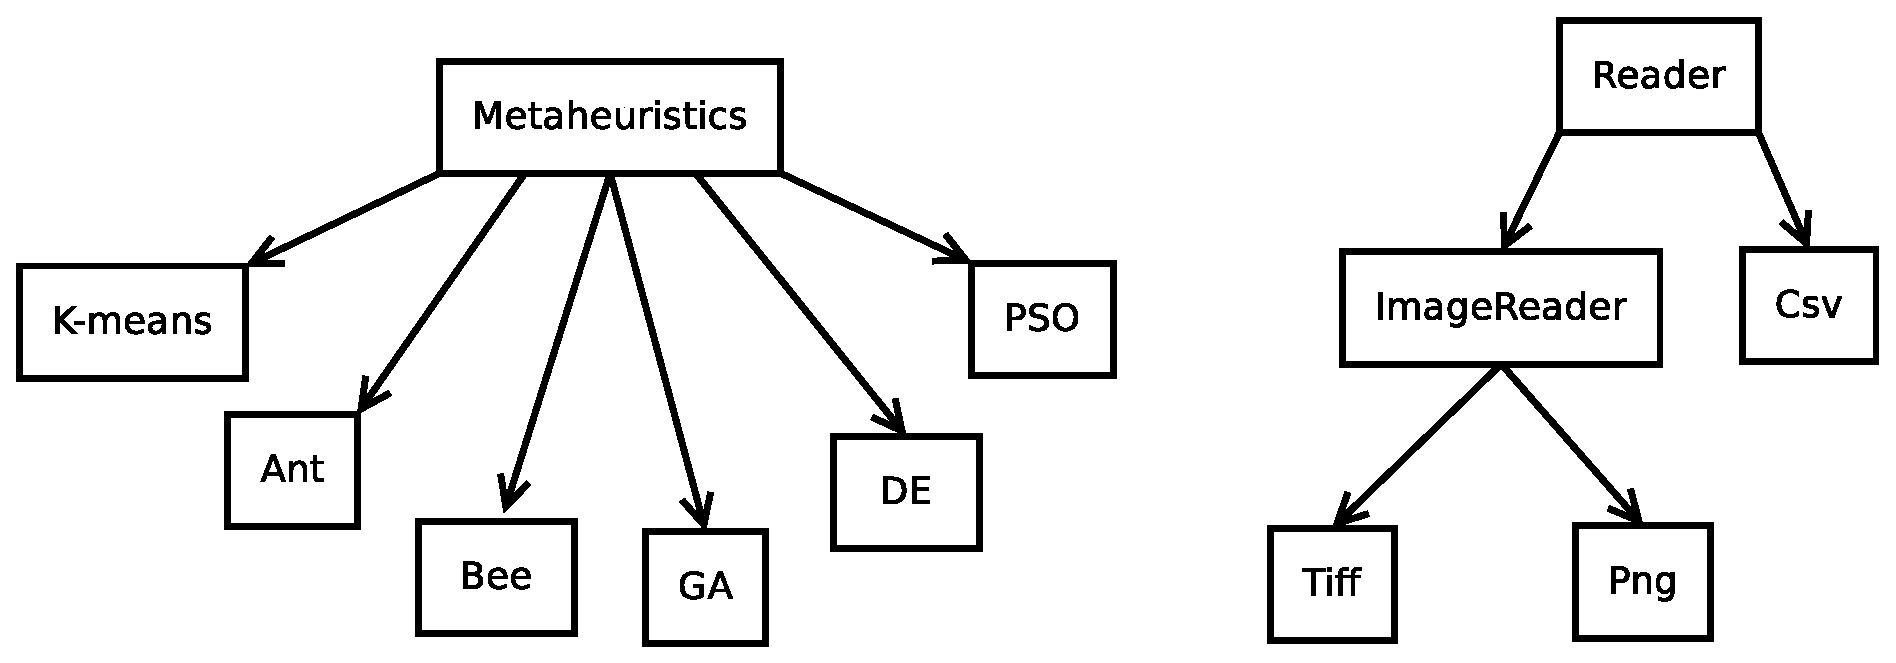
\includegraphics[scale=0.35]{figures/clases.eps}
\caption{Diagrama de clases}
\label{fig:jclases}
\end{figure}

    \emph{Metaheuristics} es una clase abstracta, que posee algunos métodos
generales compartidos por las metaheurísticas hijas. En especial, tiene dos
métodos abstractos importantes:
\begin{itemize}
    \item \emph{initialize}: Inicializa las variables necesarias para que la
metaheurística sea ejecutada.
    \item \emph{run}: Ejecuta la metaheurística.
\end{itemize}

Por otro lado, \emph{Reader} es también una clase abstracta, encargada de leer
el archivo de entrada (formato \emph{PNG} y \emph{TIFF} para las imágenes y
\emph{CSV} para archivos de datos numéricos) y escribir el archivo de salida.

\begin{comment}

\section{Máquina de pruebas} \label{sect:testbed}

    Todas las pruebas fueron realizadas con un computador cuyas características
aparecen en la tabla \ref{tb:testbed}. El programa implementado, de nombre
{\bf mhs}, fue compilado con \emph{gcc} con optimización de nivel 3 en la
máquina mencionada anteriormente. Se eligió ese nivel de optimización ya que
aplica todas las mejoras del compilador \emph{gcc}.

\begin{table}[htb]
\footnotesize
\begin{center}
\begin{tabular}{|>{\columncolor{lightgray}}c|c|}
\hline
CPU & Intel Core I5 650 \\
\hline
RAM & 6 GB \\
\hline
Distribución & Ubuntu 11.04 x86\_64 bits \\
\hline
Kernel Linux & 2.6.38-8-generic \\
\hline
Versión gcc & 4.5.2 \\
\hline
\end{tabular}
\caption{Computador usado para las pruebas}
\label{tb:testbed}
\end{center}
\end{table}

\end{comment}

\section{Métricas usadas}  \label{sect:meusada}

    Para medir la similitud entre los patrones de un conjunto de datos, se utilizó
la distancia euclidiana (ver ecuación (\ref{mdist: euclidean})), explicada
anteriormente. Fue elegida debido a su fácil implementación, buenos resultados y
rapidez.

    Se utilizaron el índice $DB$ y la cuantificación del error $J_e$ para evaluar la 
calidad de las soluciones finales de cada algoritmo implementado para compararlos
entre sí.

\section{Representación de Individuos} \label{sect:repind}

    Los algoritmos \emph{genético} y \emph{de abeja}, \emph{evolución diferencial} y
\emph{optimizador de enjambre de partículas} tienen la misma representación para
sus individuos. En la figura \ref{fig:individual}\cite{DoGeGr2007} se puede observar la representación
del vector de centroides que tiene cada individuo.

\begin{figure}[!h]
    \centering
    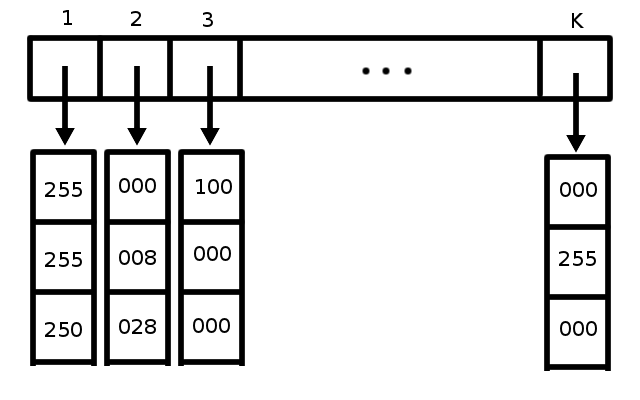
\includegraphics[scale=0.4]{figures/individual.png}
    \caption{Individuos: Vector de centroides}
    \label{fig:individual}
\end{figure}

\begin{comment}
\section{Formato de pruebas}  
\label{sect:ajustep}

    Se buscó el conjunto de mejores valores para los parámetros de cada algoritmo
implementado. Algunos de estos parámetros se mantuvieron fijos, decisión tomada
a partir de pruebas experimentales o recomendaciones de artículos y libros. Para
ello se realizaron dos conjuntos de pruebas y análisis:

\begin{enumerate}
    \item \emph{Pruebas con análisis de varianza}(ver apéndice \ref{apendiceb}):
            Para las pruebas, se recabó información de cada metaheurística de la
        siguiente forma:
        \begin{enumerate}
            \item Se generaron valores para el conjunto de parámetros de cada
        metaheurística, a partir de la permutación de rangos discretos válidos para cada
        uno de los mismos (véanse las secciones \ref{sect:iga-rv}, \ref{sect:iwpso-rv},
        \ref{sect:inpso-rv}, \ref{sect:inde-rv}, \ref{sect:isde-rv},
        \ref{sect:ibee-rv} y \ref{sect:iant-rv}).
            \item Se ejecutó cada metaheurística con cada uno de los conjunto de
        valores generados anteriormente y se extrajo el valor de la función de
        \emph{fitness} $f$ de cada solución final.
        \end{enumerate}
	\item \emph{Pruebas exhaustivas} (ver apéndice \ref{apendicea}):
            Para las pruebas, se recabó información de cada metaheurística de la
        siguiente forma:
        \begin{enumerate}
            \item Se generaron valores para el conjunto de parámetros de cada
        metaheurística a partir de la permutación de rangos discretos válidos para cada
        uno de los mismos (véanse las secciones  \ref{sect:agenetico}, \ref{sect:anpso},
        \ref{sect:awpso}, \ref{sect:ande}, \ref{sect:asde}, \ref{sect:abee},
        \ref{sect:aant}).
            \item Se ejecutó cinco veces cada metaheurística con cada uno de los     
        conjunto de valores generados anteriormente.
            \item De los resultados obtenidos, se promediaron las cinco corridas de cada
        metaheurística y se tomaron los veinte mejores conjunto de valores.
            \item Cada metaheurística fue ejecutada nuevamente con cada uno de los veinte
        mejores conjuntos de valores para ella. Fueron ejecutadas treinta veces para
        cada conjunto de valores.
        \end{enumerate}
\end{enumerate}

\subsection{Metaheurísticas híbridas}\label{exp:hibrido}

    Adicionalmente a la implementación de las metaheurísticas, también se implementaron
híbridos de éstas con el algoritmo determinista \emph{K-means}. En otras palabras,
las soluciones finales de cada metaheurística eran mejoradas por el algoritmo
\emph{K-means}.

    Se realizaron las \emph{pruebas exhaustivas} descritas anteriormente (ver
sección \ref{sect:ajustep}) tanto con las metaheurísticas híbridas como para las
no híbridas para luego hacer un análisis comparativo de las mismas (ver apéndice
\ref{apendicec}).

    Se utilizaron las metaheurísticas híbridas para hacer los análisis comparativos
del capítulo \ref{chap:analisis} ya que tuvieron mejor calidad de soluciones
finales que sus contrapartes no híbridas (ver apendice \ref{apendicec}).

\subsection{Archivos de prueba}\label{datatest}

    Las pruebas mencionadas anteriormente (ver sección \ref{sect:ajustep}) se
realizaron para los conjuntos de datos mostrados a continuación:
\begin{itemize}

\item {\bf Lenna:}\label{test:lenna}

Es una imagen muy usada por los investigadores en el área de imágenes. 
\textbf{El número óptimo de clusters está en el rango $[5,10]$\cite{OuBa2007}.}
Se usó una versión de resolución 128x128.

\begin{figure}[htb]
\centering

\includegraphics{figures/lenamini.png}
\caption{Lenna}
\label{fig:lenna}
\end{figure}

\item {\bf Iris:}\label{test:iris}

Es un conjunto bastante conocido de datos que
consiste en tres diferentes especies de la planta iris: \emph{Iris setosa},
\emph{Iris virginica} e \emph{Iris versicolour}. Para cada una de las especies,
hay 50 muestras con cuatro atributos de tipo real: longitud del sépalo, ancho
del sépalo, longitud de pétalos y ancho de pétalos. \textbf{La partición óptima
es de 3 clusters con 50 objetos cada uno, de los cuales cada cluster representa a
una de las especies \cite{SwAjAm2008}.}


\item {\bf Imagen sintética:}

Es una imagen creada con la finalidad de ver gráficamente el buen funcionamiento
de las metaheurísticas implementadas. \textbf{Al ser una imagen simple, un buen
algoritmo debería encontrar la partición óptima (7 clusters: 6 figuras bien
diferenciadas y el fondo) sin ninguna dificultad.}

\begin{figure}[htb]
\centering

\includegraphics[scale=0.3]{figures/trivial.png}
\caption{Imagen sintética}
\label{fig:Trivial}
\end{figure}

\end{itemize}

\subsection{Formato de las tablas de resultados}

    A continuación, se presentan los significados de las abreviaturas de las
cabeceras de las tablas de resultados:
\begin{itemize}
    \item \textbf{FO}: Valor de la función de \emph{fitness} $1/DB$ para la
solución final.
    \item \textbf{DB}: Valor del índice \emph{DB} para la solución final.
    \item \textbf{$J_e$}: Valor de la cuantificación del error para la solución
final.
	\item \textbf{E}:Cantidad de evaluaciones de la función de \emph{fitness}.
\end{itemize}

\end{comment}

\section{K-means}  \label{chap:ikmeans}

    Este método directo fue implementado siguiendo el pseudo-código \ref{Kmeans}
mencionado en la sección \ref{sect:cpart}, agregándole las siguientes
características:
\begin{itemize}
    \item La solución inicial es generada aleatoriamente.
    \item El algoritmo se detiene cuando no se mejora la solución en un número
dado de iteraciones.
	\item Si existe algún cluster vacío, lo elimina. Esto implica que el
algoritmo \emph{K-means} implementado puede reducir el número de clusters.
\end{itemize}
    El \emph{K-means}, al ser un método directo, tiene un comportamiento
determinista.

\begin{comment}

\subsection{Resultados obtenidos para \textbf{Lenna}}

    A continuación, se presenta una tabla resumen de 30 ejecuciones del
algoritmo \emph{K-means}:

\begin{table}[h!]
\footnotesize
\begin{center}
\begin{tabular}{|c|c|c|c|c|}
\hline
&{\bf FO}&{\bf DB}&{\bf $J_e$}\\
\hline
\hline
Promedio & 1.2037 & 0.8333 & 17.1739\\
\hline
Mejor & 1.2797 & 0.7814 & 16.9164\\
\hline
Peor & 1.0456 & 0.9564 & 17.091\\
\hline
\end{tabular}
\caption{Resultados de \emph{K-means} para {\bf Lenna}}
\label{tb:pmpkmeansimg}
\end{center}
\end{table}


\subsection{Resultados obtenidos para \textbf{Iris}}

    A continuación, se presenta una tabla resumen de 30 ejecuciones del
algoritmo \emph{K-means}:

\begin{table}[h!]
\footnotesize
\begin{center}
\begin{tabular}{|c|c|c|c|c|}
\hline
&{\bf FO}&{\bf DB}&{\bf $J_e$}\\
\hline
\hline
Promedio & 1.4915 & 0.6756 & 0.64\\
\hline
Mejor & 1.6695 & 0.599 & 0.6339\\
\hline
Peor & 0.9983 & 1.0017 & 0.7094\\
\hline
\end{tabular}
\caption{Resultados de \emph{K-means} para {\bf Lenna}}
\label{tb:pmpkmeanscsv}
\end{center}
\end{table}


\end{comment}

\section{Algoritmo Genético (\emph{GA})}  \label{sect:igenetico}

    A partir de las distintas implementaciones de algoritmo genético propuestos
en \cite{HrCaFr2009} y siguiendo el pseudo-código \ref{GA}, mencionado
anteriormente, se implementó un \emph{GA} con las si\-guien\-tes características:
\begin{itemize}
    \item El \emph{cromosoma} está representado por el vector de centroides
de cada individuo (ver sección \ref{sect:repind}). Esto permite que las operaciones 
evolutivas tengan más impacto sobre las soluciones de los mismos. Luego las soluciones 
son actualizadas a partir de los cambios hechos en los vectores de centroide como se
muestra en el pseudo-código \ref{rebuildGA}.
\begin{lstlisting}[float=h!, caption={Actualización de Soluciones}, label=rebuildGA]
- Para cada $i \in [1, N]$:
    - Si $d(\overrightarrow{z}_i, \overrightarrow{m}_k)$ es mínima,
      donde $k \in [1, K]$:
        - Introducir el patrón $\overrightarrow{z}_i$ en cluster $C_k$.
      Fin.
  Fin.
\end{lstlisting}

    \item La \emph{selección} se realiza a través de un torneo de tamaño $tt$.
Se eligen aleatoriamente $tt$ individuos de la población, de los cuales se escogen
a los dos con mejor valor de función de \emph{fitness}. Estos serán los candidatos
para \emph{cruce}. Este tipo de selección permite tener poblaciones más heterogéneas
ya que elige aleatoriamente a los individuos para el \emph{cruce}.

    \item El \emph{cruce} es el de un punto, explicado en la sección \ref{gen: point}.
De los cuatro individuos (2 padres y 2 hijos), sólo los que tengan mejor función
de \emph{fitness} se incorporarán a la población.

    \item La \emph{mutación} no es exclusiva de los hijos generados, sino de
cualquier miembro de la población, elegido aleatoriamente. Se implementaron tres
posibles tipos con la misma probabilidad de o\-cu\-rren\-cia:
    \begin{itemize}
        \item \textbf{Creación de un cluster}: se crea un nuevo centroide con un
patrón aleatorio del conjunto de datos.
        \item \textbf{Eliminación de un cluster}: se elige un centroide de manera
aleatoria y se elimina. Los elementos de este cluster son reasignados a los
demás clusters.
        \item \textbf{Cambio de un centroide}: consiste en reemplazar un centroide elegido aleatoriamente, con un patrón aleatorio del conjunto de datos.
    \end{itemize}
    Estas mutaciones permiten introducir diversidad cromosómica a la población
del algoritmo.
    \item El algortimo se detiene cuando no se mejora la solución en un
número dado de iteraciones.
\end{itemize}

    Entre las ventajas del algoritmo, destacan:
\begin{itemize}
    \item La cantidad total de clusters $K$, no tiene que ser conocida de
antemano. Basta con suministrarle una cantidad de clusters máximo.
    \item Es fácil de implementar, ya que es un algoritmo sencillo.
    \item Es fácil de entonar, ya que no tiene muchos parámetros.
\end{itemize}

\begin{comment}
\subsection{Parámetros variables}\label{sect:iga-pv}

    A continuación, se describen los parámetros variables del algoritmo:
\begin{itemize}
    \item $I$: representa a la cantidad total de individuos de la población,
donde $I \geq 2$.
    \item $tt$: representa el tamaño del torneo, donde $tt \geq 2$ y $tt \leq I$.
    \item $pc$: representa la probabilidad de cruce de los individuos y
está acotado en el rango $[0, 1]$.
    \item $pm$: representa la probabilidad de mutación de los individuos y
está acotado en el rango $[0, 1]$.
\end{itemize}

\subsubsection{Resultados obtenidos para \textbf{Lenna}}

    A continuación, se presenta una tabla resumen de 30 ejecuciones del mejor
conjunto de valores para los parámetros del algoritmo genético híbrido con
\emph{K-means} (\emph{GAH}) para la imagen \textbf{Lenna} (ver sección
\ref{exp:hibrido}):

\begin{table}[h!]
\footnotesize
\begin{center}
\begin{tabular}{|c|c|c|c|c|c|c|c|c|c|}
\hline
& {\bf FO} & {\bf DB}& $J_e$ & $I$ & $tt$ & $pc$ & $pm$ \\
\hline
\hline
Promedio   & 1.2753 & 0.7853  & 17.5582 &  &  &  & \\
\cline{1-4}
Mejor & 1.4104 & 0.709  & 19.4009 & 10 & 4 & 0.8 & 1.0\\
\cline{1-4}
Peor & 1.179 & 0.8481  & 17.6034 &  &  &  & \\\hline
\end{tabular}
\caption{Resultados de las mejores corridas de \emph{GAH} para {\bf Lenna}}
\label{tb:pmpgahibimg}
\end{center}
\end{table}


\newpage

\subsubsection{Resultados obtenidos para \textbf{Iris}}

    A continuación, se presenta una tabla resumen de 30 ejecuciones del mejor
conjunto de valores para los parámetros del algoritmo genético híbrido con
\emph{K-means} (\emph{GAH}) para el archivo de datos \textbf{Iris} (ver sección
\ref{exp:hibrido}):

\begin{table}[h!]
\footnotesize
\begin{center}
\begin{tabular}{|c|c|c|c|c|c|c|c|c|c|}
\hline
& {\bf FO} & {\bf DB}& $J_e$ & $I$ & $tt$ & $pc$ & $pm$ \\
\hline
\hline
Promedio   & 2.6521 & 0.3771  & 0.5029 &  &  &  & \\
\cline{1-4}
Mejor & 2.6521 & 0.3771  & 0.5029 & 25 & 12 & 0.2 & 1.0\\
\cline{1-4}
Peor & 2.6521 & 0.3771  & 0.5029 &  &  &  & \\\hline
\end{tabular}
\caption{Resultados de las mejores corridas de \emph{GAH} para {\bf Iris}}
\label{tb:pmpgahibcsv}
\end{center}
\end{table}


\subsubsection{Influencia de los parámetros}

Teniendo en cuenta que el \emph{rango probado} es el conjunto de valores utilizado
para las pruebas y el \emph{rango efectivo} es el conjunto valores del parámetros
para los 20 mejores resultados del algoritmo \emph{GAH} (tablas \ref{tb:tablegahibimg}
y \ref{tb:tablegahibcsv}), se encontró lo siguiente:

\begin{itemize}
    \item Para la imagen \textbf{Lenna}:
        \begin{itemize}
            \item Parámetro $I$:
                Como el \emph{rango probado} ($[5, 40]$) es
                igual al \emph{rango efectivo} ($[5, 40]$) no importa que valor tome el
                parámetro $I$, el \emph{GAH} puede dar una buena solución
                final. Por lo tanto, este parámetro no influye
                considerablemente en la bondad de la solución final.
            \item Parámetro $tt$:
                Como el \emph{rango probado}($[4, 40]$) es
                mayor al \emph{rango efectivo} ($[4, 24]$), es relevante el valor que se
                le asigne al parámetro $tt$. \textbf{Por lo tanto, este
                parámetro influye en la bondad de la solución final.}
            \item Parámetro $pc$:
                Como el \emph{rango probado}($[0.0; 1.0]$) es
                practicamente igual al \emph{rango efectivo} (sólo faltan el $0.4$ y $0.9$), 
                no importa que valor tome el
                parámetro $pc$, el \emph{GAH} puede dar una buena solución
                final. Por lo tanto, este parámetro no influye
                considerablemente en la bondad de la solución final.
            \item Parámetro $pm$:
                Como el \emph{rango probado}($[0.1; 1.0]$ ) es
                mayor al \emph{rango efectivo} ($[0.5; 1.0]$ ), es relevante el valor que se
                le asigne al parámetro $pm$. \textbf{Por lo tanto, este
                parámetro influye en la bondad de la solución final.}
        \end{itemize}
	\item Para el archivo numérico \textbf{Iris}:
        \begin{itemize}
            \item Parámetro $I$:
                Como el \emph{rango probado}($[5, 40]$) es
                mayor al \emph{rango efectivo} ($[25, 40]$), es relevante el valor que se
                le asigne al parámetro $I$. \textbf{Por lo tanto, este
                parámetro influye en la bondad de la solución final.}
			\item Para los parámetros $tt$, $pc$ y $pm$ se observa un comportamiento
				similar al encontrado para la imagen \textbf{Lenna}.
        \end{itemize}
\end{itemize}
\end{comment}

\section{Optimizador de Enjambre de Partículas (\emph{PSO})}  \label{sect:ipso}

    Se implementó el algoritmo \emph{gbest PSO}(pseudo-código \ref{PSO}), basado en la tesis doctoral de
Mahamed G. H. Omran \cite{PSO_0} con las siguientes características:
\begin{itemize}
    \item La población inicial tiene soluciones generadas aleatoriamente.
    \item El algoritmo se detiene cuando no se mejora la solución en un
número dado de iteraciones.
	\item El número de clusters no es variable. Para esto se implementó un
procedimiento que llena clusters vacíos al cambiar su centroide, descrito en
el pseudo-código \ref{sect: ipso-asig}.
\begin{lstlisting}[float=h!, caption={Asignación de nuevo centroide}, label={sect: ipso-asig}]
- Aplicar el proceso de asignación, explicado en el pseudo-código %\ref{rebuildGA}%.
- Para cada $i \in [1, K]$:
    - Si el cluster $C_i$ está vacío o tiene un sólo elemento:
        - Tomar el patrón $\overrightarrow{z} \in C_k$ que esté más alejado de su centroide $\overrightarrow{m}_k$,
          donde $k \in [1, K]$
        - Asignar al centroide $\overrightarrow{m}_i$ el patrón $\overrightarrow{z}$.
        - Aplicar el proceso de asignación, explicado en el pseudo-código %\ref{rebuildGA}%.
        - Reiniciar $i$,
      Fin.
  Fin.
\end{lstlisting}
\end{itemize}

    Se usaron dos funciones de \emph{fitness} diferentes. Ambas funciones
pertenecen a un problema de optimización de minimización. Por lo tanto, a menor
valor, mejor solución.
    
\subsection{Función de \emph{fitness} con pesos (\emph{WPSO})}\label{sect:iwpso}

    El \emph{WPSO} tiene la siguiente función de \emph{fitness} \cite{PSO_0}:
\begin{equation}\label{pso: wpso}
    f(x_i) = w_1 \cdot \overline{d}_{Max}(x_i) + w_2 \cdot (Z_{Max} - d_{Min}(x_i)) + w_3 \cdot J_e
\end{equation}
donde,
\begin{itemize}
    \item $Z_{Max}$ es la distancia máxima entre el patrón con valores de
atributos máximos y el patrón con valores de atributos mínimos.
    \item $\overline{d}_{Max}(x_i)$ es la distancia máxima promedio de la
distancia entre un patrón y el centroide del cluster al que pertenece. Mientras
más pequeña sea esta distancia, los clusters son más densos:
\begin{equation}\label{pso: dmax}
    \overline{d}_{Max}(x_i) = \displaystyle\max_{k \in [1,K]} \left[\displaystyle\sum_{\forall \overrightarrow{z} \in C_{i,k}} \displaystyle\frac{d(\overrightarrow{z}, \overrightarrow{m}_{i,k})}{N_{i,k}}\right]
\end{equation}
donde $z$ es un patrón del conjunto de datos.
    \item $\overline{d}_{Min}(x_i)$ es la distancia mínima entre los centroides
de cada clusters. Mientras más grande sea esta distancia, mejor diferenciados
estarán los clusters:
\begin{equation}\label{pso: dmin}
    d_{Min}(x_i) = \displaystyle\min_{k \in [1,K]} d(\overrightarrow{m}_{i,k}, \overrightarrow{m}_{i,l}); \forall k,l \in \{1, \cdots, K\},k \neq l
\end{equation}
    \item $J_e$ es la cuantificación del error (\ref{cluster: je}).
    \item $w_1$ es el peso de la distancia \emph{intra-cluster}. El sub-objetivo
del algoritmo es hacer que esta distancia sea mínima.
    \item $w_2$ es el peso de la distancia \emph{inter-cluster}. El sub-objetivo
del algoritmo es hacer que esta distancia sea máxima.
    \item $w_3$ es el peso de la cuantificación del error. El sub-objetivo del
algoritmo es hacer que el error sea mínimo.
\end{itemize}

    La principal ventaja de esta función de \emph{fitness} es la de poder
controlar los diferentes sub-objetivos de clustering de manera independiente a
través de los valores de los pesos.
\begin{comment}
\subsection{Parámetros variables}\label{sect:iwpso-pv}

    A continuación, se describen los parámetros variables del algoritmo:
\begin{itemize}
    \item $I$: representa a la cantidad total de partículas del enjambre,
donde $I \geq 2$.
    \item $w_1$, $w_2$ y $w_3$: son los pesos de la función de \emph{fitness}
(\ref{pso: wpso}), deben ser positivos y su suma debe ser igual a 1.
    \item $W$, $c_1$ y $c_2$: representan al peso inercial, factor de aprendizaje
colectivo y factor de aprendizaje social, respectivamente, descritos en la
sección \ref{sect:metapso-vel}. $W$ debe estar acotado en el rango $[0, 2]$ y
$c_1$ y $c_2$ deben satisfacer la inecuación (\ref{pso: convergece}).
    \item $vmx$: es un escalar, acotado en el rango $[0, 1]$, que multiplica al
vector $Z_{max}$ con el fin de regular la velocidad máxima de la partícula,
donde $vmx \cdot Z_{max}$ es el valor máximo de la velocidad $v(t)$ (véase la
ecuación (\ref{pso: vi})).
\end{itemize}

\subsubsection{Resultados obtenidos para \textbf{Lenna}}
    A continuación, se presenta una tabla resumen de 30 ejecuciones del mejor
conjunto de valores para los parámetros del \emph{WPSO} híbrido con
\emph{K-means} (\emph{WPSOH}) para la imagen \textbf{Lenna} (ver sección
\ref{exp:hibrido}):

\begin{table}[h!]
\footnotesize
\begin{center}
\begin{tabular}{|c|c|c|c|c|c|c|c|c|c|c|c|c|c|}
\hline
& {\bf FO} & {\bf DB}& $J_e$ & $I$ & $w_1$ & $w_2$ & $w_3$ & $W$ & $c_1$ & $c_2$ & $vmx$ \\
\hline
\hline
Promedio   & 1.2005 & 0.8348  & 17.7634 &  &  &  &  &  &  &  & \\
\cline{1-4}
Mejor & 1.3039 & 0.7669  & 16.9839 & 35 & 0.0 & 1.0 & 0.0 & 0.5 & 2.0 & 0.5 & 0.5\\
\cline{1-4}
Peor & 1.1074 & 0.903  & 17.6885 &  &  &  &  &  &  &  & \\\hline
\end{tabular}
\caption{Resultados de las mejores corridas de \emph{WPSOH} para {\bf Lenna}}
\label{tb:pmpwpsohibimg}
\end{center}
\end{table}


\subsubsection{Resultados obtenidos para \textbf{Iris}}

    A continuación, se presenta una tabla resumen de 30 ejecuciones del mejor
conjunto de valores para los parámetros del \emph{WPSO} híbrido con
\emph{K-means} (\emph{WPSOH}) para el archivo de datos \textbf{Iris} (ver sección
\ref{exp:hibrido}):

\begin{table}[h!]
\footnotesize
\begin{center}
\begin{tabular}{|c|c|c|c|c|c|c|c|c|c|c|c|c|c|}
\hline
& {\bf FO} & {\bf DB}& $J_e$ & $I$ & $w_1$ & $w_2$ & $w_3$ & $W$ & $c_1$ & $c_2$ & $vmx$ \\
\hline
\hline
Promedio   & 1.5694 & 0.6385  & 0.661 &  &  &  &  &  &  &  & \\
\cline{1-4}
Mejor & 1.6992 & 0.5885  & 0.6709 & 10 & 0.8 & 0.2 & 0.0 & 0.8 & 1.1 & 1.1 & 0.5\\
\cline{1-4}
Peor & 1.5165 & 0.6594  & 0.6466 &  &  &  &  &  &  &  & \\\hline
\end{tabular}
\caption{Resultados de las mejores corridas de \emph{WPSOH} para {\bf Iris}}
\label{tb:pmpwpsohibcsv}
\end{center}
\end{table}


\subsubsection{Influencia de los parámetros}

Teniendo en cuenta que el \emph{rango probado} es el conjunto de valores utilizado
para las pruebas y el \emph{rango efectivo} es el conjunto valores del parámetros
para los 20 mejores resultados del algoritmo \emph{WPSOH} (tablas \ref{tb:tablewpsohibimg}
y \ref{tb:tablewpsohibcsv}), se encontró lo siguiente:

\begin{itemize}
	\item Para la imagen \textbf{Lenna}:
	\begin{itemize}
		\item No se puede encontrar una relación entre los valores de los
			parámetros y el valor de la función de \emph{fitness}. Se
			puede observar que para cada parámetro el \emph{rango efectivo}
			es similar \emph{rango probado}. Esto indica que el valor que tome cada
			uno de los parámetros del algoritmo parece no tener una gran influencia en la
			solución final.
	\end{itemize}
	\item Para el archivo numérico \textbf{Iris}:
	\begin{itemize}
		\item Se puede observar que los parámetros $I$, $w_1$, $w_2$, $w_3$ y
			$W$ pueden ser fijados en $10$, $0.8$, $0.2$, $0.0$ y $0.8$,
			respectivamente. Los demás parámetros se comportan de manera similar 
			a como lo hacen para la imagen {\bf Lenna}.
	\end{itemize}
\end{itemize}

\end{comment}

\subsection{Función de \emph{fitness} sin pesos (\emph{NPSO})}\label{sect:inpso}
    El \emph{NPSO} tiene la siguiente función de \emph{fitness} \cite{PSO_0}:
\begin{equation}\label{pso: npso}
    f(x_i) = \displaystyle \frac{\displaystyle\frac{\overline{d}_{Max}(x_i)}{2 \cdot Z_{Max}} + \frac{J_e}{2 \cdot Z_{Max}}}{\displaystyle\frac{d_{Min}(x_i)}{Z_{Max}}}
\end{equation}

    Los términos $\overline{d}_{Max}(x_i)$ y $J_e$ están normalizados de modo que
pertenezcan al intervalo $[0, \frac{1}{2}]$, mientras el término $d_{Min}(x_i)$
está normalizado para pertenecer al intervalo $(0, 1]$. Así que esta función de
\emph{fitness} está acotada en el intervalo $[0, 1]$.

    La ventaja principal de esta función de \emph{fitness} es que prescinde de
los pesos de la función (\ref{pso: wpso}), de modo que se facilita la
entonación del algoritmo.

\begin{comment}
\subsection{Parámetros variables}\label{sect:inpso-pv}

    Los parámetros variables son los mismos descritos en la sección \ref{sect:iwpso-pv},
exceptuando los pesos $w_1$, $w_2$ y $w_3$.

\subsubsection{Resultados obtenidos para \textbf{Lenna}}
    A continuación, se presenta una tabla resumen de 30 ejecuciones del mejor
conjunto de valores para los parámetros del \emph{NPSO} híbrido con
\emph{K-means} (\emph{NPSOH}) para la imagen \textbf{Lenna} (ver sección
\ref{exp:hibrido}):

\begin{table}[h!]
\footnotesize
\begin{center}
\begin{tabular}{|c|c|c|c|c|c|c|c|c|c|c|}
\hline
& {\bf FO} & {\bf DB}& $J_e$ & $I$ & W & $c_1$ & $c_2$ & $vmx$ \\
\hline
\hline
Promedio   & 1.2071 & 0.8297  & 17.5799 & &  &  &  & \\
\cline{1-4}
Mejor & 1.2968 & 0.7711  & 17.3749 & 35 & 0.8 & 1.7 & 1.7 & 0.5\\
\cline{1-4}
Peor & 1.1113 & 0.8999  & 19.3463 &  &  &  &  & \\\hline
\end{tabular}
\caption{Resultados de las mejores corridas de \emph{NPSOH} para {\bf Lenna}}
\label{tb:pmppsohibimg}
\end{center}
\end{table}


\subsubsection{Resultados obtenidos para \textbf{Iris}}

    A continuación, se presenta una tabla resumen de 30 ejecuciones del mejor
conjunto de valores para los parámetros del \emph{NPSO} híbrido con
\emph{K-means} (\emph{NPSOH}) para el archivo de datos \textbf{Iris} (ver sección
\ref{exp:hibrido}):

\begin{table}[h!]
\footnotesize
\begin{center}
\begin{tabular}{|c|c|c|c|c|c|c|c|c|c|c|}
\hline
& {\bf FO} & {\bf DB}& $J_e$ & $I$ & W & $c_1$ & $c_2$ & $vmx$ \\
\hline
\hline
Promedio   & 1.5654 & 0.6395  & 0.6606 &  &  &  &  & \\
\cline{1-4}
Mejor & 1.6626 & 0.6015  & 0.6807 & 25 & 1.1 & 1.7 & 0.5 & 0.5\\
\cline{1-4}
Peor & 1.5006 & 0.6664  & 0.649 &  &  &  &  & \\\hline
\end{tabular}
\caption{Resultados de las mejores corridas de \emph{NPSOH} para {\bf Iris}}
\label{tb:pmppsohibcsv}
\end{center}
\end{table}


\subsubsection{Influencia de los parámetros}

Teniendo en cuenta que el \emph{rango probado} es el conjunto de valores utilizado
para las pruebas y el \emph{rango efectivo} es el conjunto valores del parámetros
para los 20 mejores resultados del algoritmo \emph{NPSOH} (tablas \ref{tb:tablepsohibimg}
y \ref{tb:tablepsohibcsv}), se encontró lo siguiente:

\begin{itemize}
	\item Para la imagen \textbf{Lenna}:
	\begin{itemize}
		\item No se puede encontrar una relación entre los valores de los
			parámetros y el valor de la función de \emph{fitness}. Se
			puede observar que para cada parámetro el \emph{rango efectivo}
			es similar \emph{rango probado}. Esto indica que el valor que tome cada
			uno de los parámetros del algoritmo parece no tener una gran influencia en la
			solución final.
	\end{itemize}
	\item Para el archivo numérico \textbf{Iris}:
	\begin{itemize}
		\item Se puede observar que los parámetros $I$ y $W$ pueden ser fijados
			en $25$ y $1.1$, respectivamente. Los demás parámetros se comportan de manera similar 
			a como lo hacen para la imagen {\bf Lenna}.
	\end{itemize}
\end{itemize}

\end{comment}

\section{Evolución Diferencial (\emph{DE})}  \label{sect:ide}

    Esta metaheurística fue implementada siguiendo el pseudo-código \ref{DE}, 
mencionado anteriormente en la sección \ref{sect:metade}, con la
función objetivo del \emph{WPSO} (\ref{sect:iwpso}) y
el procedimiento que mantiene la cantidad de clusters fijo \ref{sect: ipso-asig}. Sin embargo, tiene
varias diferencias basadas en los trabajos \cite{SwAjAm2008} y \cite{OmEnSa2005}.
A continuación, se presentan las modificaciones:

\begin{itemize}
    \item El hijo generado a partir del \emph{cruce} será diferente al padre en
al menos un atributo.
    \item El algoritmo se detiene al alcanzar el máximo número de iteraciones
$maxit$.
\end{itemize}

\subsection{Parámetros variables}\label{sect:isde-pv} \label{sect:inde-pv}

    A continuación, se describen los parámetros variables del algoritmo:
\begin{itemize}
    \item $I$: representa a la cantidad total de individuos.
    \item $w_1$, $w_2$ y $w_3$: son los pesos de la función de \emph{fitness}
(\ref{pso: wpso}), deben ser positivos y su suma debe ser igual a 1.
    \item $\gamma$: factor de escalado de la diferencia.
    \item $Cr$: representa la probabilidad de cruce  de los individuos.
\end{itemize}

    Los parámetros $\gamma$ y $Cr$ pueden ser provistos por el usuario (\emph{SDE})
o calculados automáticamente durante la ejecución de la metaheurística
(\emph{NDE}).

    En el caso del \emph{NDE}, los parámetros son calculados de la siguiente
forma\cite{SwAjAm2008}: 

\begin{itemize}

\item $\gamma$: En cada iteración del algoritmo, se calcula un nuevo valor para
$\gamma$ de la siguiente forma:
\begin{equation}\label{de: gamma}
    0.5 \cdot ( 1 + rand(0,1) )
\end{equation}
donde $rand(0,1)$ es un número aleatorio en el intervalo $[0, 1]$. La media de los
valores generados será 0.75, permitiendo variaciones estocásticas en los vectores
hijo generados. Esto ayuda a mantener diversidad en la población.

\item $Cr$: Se establece una probabilidad de cruce máxima $Cr_{max}$ y una probabilidad
de cruce mínima $Cr_{min}$. En cada iteración del algoritmo, la variable $Cr$ se
decrementará linealmente dentro del rango $[Cr_{min}, Cr_{max}]$. A medida que
el valor de $Cr$ disminuye, heredarán más atributos del padre. La variación del
parámetro $Cr$ está dado por:
\begin{equation}\label{de: cr}
    Cr_i = (Cr_{max}-Cr_{min}) \cdot \displaystyle\frac{maxit - i}{maxit} + Cr_{min}
\end{equation}
donde $Cr_i$ es la probabilidad de cruce $Cr$ en la iteración $i$ y $maxit$ es el
número máximo de iteraciones del algoritmo. En la implementación del \emph{NDEH},
se tomaron $Cr_{max} = 1$ y $Cr_{min} = 0.5$
\end{itemize}

\begin{comment}

\subsubsection{Resultados obtenidos para \textbf{Lenna} (\emph{SDE})}
    A continuación, se presenta una tabla resumen de 30 ejecuciones del mejor
conjunto de valores para los parámetros del \emph{SDE} híbrido con
\emph{K-means} (\emph{SDEH}) para la imagen \textbf{Lenna} (ver sección
\ref{exp:hibrido}):

\begin{table}[h!]
\footnotesize
\begin{center}
\begin{tabular}{|c|c|c|c|c|c|c|c|c|c|c|c|}
\hline
& {\bf FO} & {\bf DB}& $J_e$ & $I$ & $w_1$ & $w_2$ & $w_3$ & $\gamma$ & $Cr$ \\
\hline
\hline
Promedio   & 1.1813 & 0.8491  & 19.5178 &  &  &  &  &  & \\
\cline{1-4}
Mejor & 1.3195 & 0.7578  & 16.9559 & 10 & 0.4 & 0.5 & 0.1 & 0.5 & 0.7\\
\cline{1-4}
Peor & 0.9948 & 1.0052  & 39.0413 &  &  &  &  &  & \\\hline
\end{tabular}
\caption{Resultados de las mejores corridas de \emph{SDEH} para {\bf Lenna}}
\label{tb:pmpsdehibimg}
\end{center}
\end{table}


\subsubsection{Resultados obtenidos para \textbf{Iris} (\emph{SDE})}

    A continuación, se presenta una tabla resumen de 30 ejecuciones del mejor
conjunto de valores para los parámetros del \emph{SDE} híbrido con
\emph{K-means} (\emph{SDEH}) para el archivo de datos \textbf{Iris} (ver sección
\ref{exp:hibrido}):

\begin{table}[h!]
\footnotesize
\begin{center}
\begin{tabular}{|c|c|c|c|c|c|c|c|c|c|c|c|}
\hline
& {\bf FO} & {\bf DB}& $J_e$ & $I$ & $w_1$ & $w_2$ & $w_3$ & $\gamma$ & $Cr$ \\
\hline
\hline
Promedio   & 1.5312 & 0.6533  & 0.6448 &  &  &  &  &  & \\
\cline{1-4}
Mejor & 1.5778 & 0.6338  & 0.625 & 15 & 0.5 & 0.1 & 0.4 & 0.8 & 0.9\\
\cline{1-4}
Peor & 1.5006 & 0.6664  & 0.649 &  &  &  &  &  & \\\hline
\end{tabular}
\caption{Resultados de las mejores corridas de \emph{SDEH} para {\bf Iris}}
\label{tb:pmpsdehibcsv}
\end{center}
\end{table}


\subsubsection{Resultados obtenidos para \textbf{Lenna} (\emph{NDE})}

    A continuación, se presenta una tabla resumen de 30 ejecuciones del mejor
conjunto de valores para los parámetros del \emph{NDE} híbrido con
\emph{K-means} (\emph{NDEH}) para la imagen \textbf{Lenna} (ver sección
\ref{exp:hibrido}):

\begin{table}[h!]
\footnotesize
\begin{center}
\begin{tabular}{|c|c|c|c|c|c|c|c|c|c|}
\hline
& {\bf FO} & {\bf DB}& $J_e$ & $I$ & $w_1$ & $w_2$ & $w_3$ \\
\hline
\hline
Promedio   & 1.2132 & 0.8256  & 19.9024 &  &  &  & \\
\cline{1-4}
Mejor & 1.3346 & 0.7493  & 16.589 & 40 & 0.0 & 0.0 & 1.0\\
\cline{1-4}
Peor & 1.1097 & 0.9011  & 17.6334 &  &  &  & \\\hline
\end{tabular}
\caption{Resultados de las mejores corridas de \emph{NDEH} para {\bf Lenna}}
\label{tb:pmpdehibimg}
\end{center}
\end{table}


\subsubsection{Resultados obtenidos para \textbf{Iris} (\emph{NDE})}

    A continuación, se presenta una tabla resumen de 30 ejecuciones del mejor
conjunto de valores para los parámetros del \emph{NDE} híbrido con
\emph{K-means} (\emph{NDEH}) para el archivo de datos \textbf{Iris} (ver sección
\ref{exp:hibrido}):

\begin{table}[h!]
\footnotesize
\begin{center}
\begin{tabular}{|c|c|c|c|c|c|c|c|c|c|}
\hline
& {\bf FO} & {\bf DB}& $J_e$ & $I$ & $w_1$ & $w_2$ & $w_3$ \\
\hline
\hline
Promedio   & 1.5638 & 0.6403  & 0.6367 &  &  &  & \\
\cline{1-4}
Mejor & 1.7153 & 0.583  & 0.6586 & 15 & 0.2 & 0.7 & 0.1\\
\cline{1-4}
Peor & 1.5006 & 0.6664  & 0.649 &  &  &  & \\\hline
\end{tabular}
\caption{Resultados de las mejores corridas de \emph{NDEH} para {\bf Iris}}
\label{tb:pmpdehibcsv}
\end{center}
\end{table}


\subsubsection{Influencia de los parámetros}

Teniendo en cuenta que el \emph{rango probado} es el conjunto de valores utilizado
para las pruebas y el \emph{rango efectivo} es el conjunto valores del parámetros
para los 20 mejores resultados del algoritmo \emph{NDEH} (tablas \ref{tb:tabledehibimg}
y \ref{tb:tabledehibcsv}), se encontró lo siguiente:

\begin{itemize}
    \item Para la imagen {\bf Lenna}:
		\begin{itemize}
		    \item Para los parámetros $I$, $w_1$ y $w_3$ el \emph{rango efectivo}
				  es similar \emph{rango probado}. Esto
		          puede indicar que no influyen considerablemente en la calidad
		          de las soluciones finales.
		    \item Parámetro $w_2$:
		          Como el \emph{rango probado}($[0.1; 1.0]$) es
		          mayor al \emph{rango efectivo} ($[0.0;0.6]$), es relevante el valor que se
		          le asigne al parámetro $w_2$. \textbf{Por lo tanto, este
		          parámetro influye en la bondad de la solución final.}
		\end{itemize}
    \item Para el archivo numérico {\bf Iris}:
		\begin{itemize}
		    \item A diferencia de los resultados para \emph{Lenna}, ningún
		    parámetro parece influir considerablemente en la calidad de las
		    soluciones finales.
		\end{itemize}
\end{itemize}

Por otro lado, teniendo en cuenta que el \emph{rango probado} es el conjunto de valores utilizado
para las pruebas y el \emph{rango efectivo} es el conjunto valores del parámetros
para los 20 mejores resultados del algoritmo \emph{SDEH} (tablas \ref{tb:tablesdehibimg}
y \ref{tb:tablesdehibcsv}), se encontró lo siguiente:

\begin{itemize}
    \item Para la imagen {\bf Lenna}:
		\begin{itemize}
		    \item Para los parámetros $I$, $w_1$ y $w_3$ el \emph{rango efectivo}
				  es similar \emph{rango probado}. Esto
				  puede indicar que no influyen considerablemente en la calidad
				  de las soluciones finales.
		    \item Para los parámetros $\gamma$ y $Cr$  el \emph{rango efectivo} 
		          posee una gran cantidad de valores del \emph{rango probado}.
		          Esto puede indicar que no influyen considerablemente en la
		          calidad de las soluciones finales.
		    \item Parámetro $w_2$:
		          Como el \emph{rango probado}($[0.1; 1.0]$) es
		          mayor al \emph{rango efectivo} ($[0.0;0.8]$), es relevante el valor que se
		          le asigne al parámetro $w_2$. \textbf{Por lo tanto, este
		          parámetro influye en la bondad de la solución final.}
	    \end{itemize}
    
    \item Para el archivo numérico {\bf Iris}:
		\begin{itemize}
			\item Se puede observar que los parámetros $I$, $w_1$, $w_2$ y $w_3$
			  	  pueden ser fijados en  $15$, $0.5$, $0.1$ y $0.4$,
				  respectivamente. 
		    \item Parámetro $\gamma$:
		          Como el \emph{rango probado}($[0.5; 1.0]$) es
		          mayor al \emph{rango efectivo} ($[0.5;0.8]$), es relevante el valor que se
		          le asigne al parámetro $\gamma$. Además, mientras más alto
		          sea su valor, mejor es el valor de la función de \emph{fitness}.
		           \textbf{Por lo tanto, este
		          parámetro influye en la bondad de la solución final.}
		    \item Parámetro $Cr$:
		    	  Tiene un comportamiento similar al obtenido con \textbf{Lenna}.
		\end{itemize}
\end{itemize}

\end{comment}

\begin{comment}
	A partir de los resultados de los 20 mejores conjuntos de valores
(tablas \ref{tb:tabledeimgfull} y \ref{tb:tabledecsvfull}) para los parámetros del
\emph{NDE}, se encontró lo siguiente:
    \begin{itemize}
        \item Para la imagen {\bf Lenna}:
        \begin{itemize}
            \item En los resultados (tabla \ref{tb:tabledeimgfull}), los parámetros
                  $I$, $w_1$ y $w_3$ poseen una gran cantidad de valores en los
                  rangos probados (sección \ref{sect:ande}). Esto
                  puede indicar que no influyen considerablemente en la calidad
                  de las soluciones finales.
            \item El parámetro $w_2$ está en el rango $[0.0;0.6]$ para los resultados
                  (tabla \ref{tb:tabledeimgfull}), el cual es de menor
                  cardinalidad que el rango (sección \ref{sect:ande}) de valores
                  probados. Por lo tanto, valores menores a $0.6$ para $w_2$
                  podrían conducir a buenas soluciones. Así que su valor influye
                  en la bondad de la solución final.
        \end{itemize}
        
        \item Para el archivo numérico {\bf Iris}:
        \begin{itemize}
            \item A diferencia de los resultados para \emph{Lenna}, ningún
            parámetro parece influir considerablemente en la calidad de las
            soluciones finales (tabla \ref{tb:tabledecsvfull}).
        \end{itemize}

    \end{itemize}

	Por otro lado, de los resultados de los 20 mejores conjuntos de valores
(tablas \ref{tb:tablesdeimgfull} y \ref{tb:tablesdecsvfull}) para los parámetros del
\emph{SDE}, se encontró lo siguiente:
    \begin{itemize}
        \item Para la imagen {\bf Lenna}:
        \begin{itemize}
            \item De manera similar al \emph{NDE}, los parámetros
                  $I$, $w_1$ y $w_3$ no parecen tener una gran influencia en la
                  calidad de las soluciones finales (tabla \ref{tb:tablesdeimgfull}).
            \item Los parámetros $\gamma$ y $Cr$ poseen una gran cantidad de
                  valores en los rangos probados (sección \ref{sect:asde}).
                  Esto puede indicar que no influyen considerablemente en la
                  calidad de las soluciones finales (tabla \ref{tb:tablesdeimgfull}).
            \item El parámetro $w_2$ está en el rango $[0.0;0.8]$ para los resultados
                  (tabla \ref{tb:tablesdeimgfull}), el cual es de menor
                  cardinalidad que el rango de valores probados (sección \ref{sect:asde}).
                  Por lo tanto, valores menores a $0.8$ para $w_2$
                  podrían conducir a buenas soluciones. Así que su valor influye
                  en la bondad de la solución final.
        \end{itemize}
        
        \item Para el archivo numérico {\bf Iris}:
        \begin{itemize}
            \item Se puede observar que los parámetros $I$, $w_1$, $w_2$ y $w_3$
                  en $15$, $0.5$, $0.1$ y $0.4$, respectivamente (tabla \ref{tb:tablesdecsvfull}).
            \item En los resultados (tabla \ref{tb:tablesdecsvfull}), $\gamma$
                  se encuentra en el rango $[0.5;0.8]$. Además, mientras más alto
                  sea su valor, mejor es el valor de la función de \emph{fitness}.
                  Esto indica que este parámetro tiene una considerable
                  influencia en la función de \emph{fitness} para \textbf{Iris}.
            \item El parámetro $Cr$ tiene un comportamiento similar al obtenido
                  con \textbf{Lenna}.
        \end{itemize}
    \end{itemize}
\end{comment}

\section{Algoritmo de Abeja (\emph{Bee})}  \label{sect:ibee}

    Esta metaheurística fue implementada siguiendo el pseudo-código \ref{Bee}
mencionado anteriormente en la sección \ref{sect:metabee}, agregándole las siguientes
características:
\begin{itemize}
    \item La población inicial de abejas tienen soluciones generadas
aleatoriamente.
    \item El algoritmo se detiene cuando no se mejora la solución en un número
dado de iteraciones.
    \item La selección de los mejores sitios se hace a partir del valor de
la función de \emph{fitness}.
    \item La búsqueda en vecindad es realizada como se puede observar en 
el pseudo-código \ref{neighbor}.
\begin{lstlisting}[float=h!, caption={Búsqueda en vecindad}, label=neighbor]
- Se elige un elemento del conjunto de datos de manera aleatoria.
- Se reemplaza el elemento elegido por el centroide del cluster al que
  pertenece.
- Se generan las nuevas soluciones con el pseudo-código %\ref{rebuildGA}%.
\end{lstlisting}
\end{itemize}

\begin{comment}
\subsection{Parámetros variables}\label{sect:ibee-pv}

    A continuación, se describen los parámetros variables del algoritmo:
\begin{itemize}
    \item $I$: Representa a la cantidad total de abejas del enjambre,
donde $I \geq 2$.
    \item $m$: Representa los sitios de flores totales, donde $m < I$.
    \item $e$: Representa los sitios de flores élite, donde $e < m$.
    \item $eb$ y $ob$: Representan la cantidad de abejas élite y la cantidad de
abejas exploradoras, respectivamente, donde $eb + ob \leq I$.
\end{itemize}

\subsubsection{Resultados obtenidos para \textbf{Lenna}}

    A continuación, se presenta una tabla resumen de 30 ejecuciones del mejor
conjunto de valores para los parámetros del \emph{Bee} híbrido con
\emph{K-means} (\emph{BeeH}) para la imagen \textbf{Lenna} (ver sección
\ref{exp:hibrido}):

\begin{table}[h!]
\footnotesize
\begin{center}
\begin{tabular}{|c|c|c|c|c|c|c|c|c|c|c|}
\hline
& {\bf FO} & {\bf DB}& $J_e$ & $I$ & $m$ & $e$ & $eb$ & $ob$ \\
\hline
\hline
Promedio   & 1.3052 & 0.7664  & 16.924 &  &  &  &  & \\
\cline{1-4}
Mejor & 1.3624 & 0.734  & 16.9922 & 35 & 15 & 2 & 14 & 6\\
\cline{1-4}
Peor & 1.2586 & 0.7945  & 16.7638 &    &  &  &  & \\\hline
\end{tabular}
\caption{Resultados de las mejores corridas de \emph{BeeH} para {\bf Lenna}}
\label{tb:pmpbeehibimg}
\end{center}
\end{table}


\subsubsection{Resultados obtenidos para \textbf{Iris}}

    A continuación, se presenta una tabla resumen de 30 ejecuciones del mejor
conjunto de valores para los parámetros del \emph{Bee} híbrido con
\emph{K-means} (\emph{BeeH}) para el archivo de datos \textbf{Iris} (ver sección
\ref{exp:hibrido}):

\begin{table}[h!]
\footnotesize
\begin{center}
\begin{tabular}{|c|c|c|c|c|c|c|c|c|c|c|}
\hline
& {\bf FO} & {\bf DB}& $J_e$ & $I$ & $m$ & $e$ & $eb$ & $ob$ \\
\hline
\hline
Promedio   & 1.9167 & 0.5412  & 0.6281 &  &  &  &  & \\
\cline{1-4}
Mejor & 2.6521 & 0.3771  & 0.5029 & 30 & 15 & 12 & 6 & 9\\
\cline{1-4}
Peor & 1.6451 & 0.6079  & 0.6287 &  &  &  &  & \\\hline
\end{tabular}
\caption{Resultados de las mejores corridas de \emph{BeeH} para {\bf Iris}}
\label{tb:pmpbeehibcsv}
\end{center}
\end{table}


\subsubsection{Influencia de los parámetros}

Teniendo en cuenta que el \emph{rango probado} es el conjunto de valores utilizado
para las pruebas y el \emph{rango efectivo} es el conjunto valores del parámetros
para los 20 mejores resultados del algoritmo \emph{BeeH} (tablas \ref{tb:tabledehibimg}
y \ref{tb:tabledehibcsv}), se encontró lo siguiente:

\begin{itemize}
        \item Para la imagen {\bf Lenna}:
	        \begin{itemize}
		        \item Parámetro $I$:
		            Como el \emph{rango probado} ($[5, 40]$) es
		            mayor al \emph{rango efectivo} ($[25, 40]$) , es relevante el valor que se
		            le asigne al parámetro $I$. \textbf{Por lo tanto, este
		            parámetro influye en la bondad de la solución final.}
		            considerablemente en la bondad de la solución final.
		        \item Parámetro $m$:
		        	Es mayor o igual a 7,
					aunque la mayor parte de los datos se encuentra en el rango $[11, 15]$.
					De tal forma el \emph{rango probado} ($[5, 15]$) es
		            mayor al \emph{rango efectivo}, generando que sea relevante el valor que se
		            le asigne al parámetro $m$. \textbf{Por lo tanto, este
		            parámetro influye en la bondad de la solución final.}
		        \item Parámetro $e$:
		            Como el \emph{rango probado}($[1,15]$) es
		            mayor al \emph{rango efectivo} ($[1,5]$), es relevante el valor que se
		            le asigne al parámetro $e$. \textbf{Por lo tanto, este
		            parámetro influye en la bondad de la solución final.}
		        \item Parámetro $eb$:
					Está en el rango $[10, 15]$, con ciertas excepciones.
					De tal forma el \emph{rango probado} ($[5, 15]$) es
		            mayor al \emph{rango efectivo}, generando que sea relevante el valor que se
		            le asigne al parámetro $eb$. Lo cual indica que con
					una cantidad de abejas élite menor a 10, la solución final tiende a desmejorar.
					\textbf{Por lo tanto, este parámetro influye en la bondad de la solución final.} 
		        \item Parámetro $ob$:
		            Como el \emph{rango probado}($[1,15]$) es
		            practicamente igual al \emph{rango efectivo} (sólo faltan el $3$, $10$, $11$ y $14$), 
		            no importa que valor tome el
		            parámetro $pc$, el \emph{BeeH} puede dar una buena solución
		            final. Por lo tanto, este parámetro no influye
		            considerablemente en la bondad de la solución final.
            \end{itemize}
        \item Para el archivo numérico {\bf Iris}:
		    \begin{itemize}
		        \item Los parámetros $I$, $m$, $e$ y $ob$ conservan el mismo comportamiento
					  que para la imagen \textbf{Lenna}. Sin embargo, el parámetro $eb$ no parece
					  mostrar el mismo patrón mostrado para las corridas de la imagen. Por lo tanto,
				  	  es posible que el valor de $eb$ no tenga tanta influencia en la bondad de la
					  solución final para el archivo numérico \textbf{Iris}.
		    \end{itemize}
\end{itemize}

\end{comment}

\begin{comment}
	A partir de los resultados de los 20 mejores conjuntos de valores
(tablas \ref{tb:tablebeeimgfull} y \ref{tb:tablebeecsvfull}) para los parámetros del
\emph{Bee}, se encontró lo siguiente:

    \begin{itemize}
        \item Para la imagen {\bf Lenna}:
        \begin{itemize}
			\item El parámetro $I$ está en el rango $[25, 40]$ para los resultados (tabla \ref{tb:tablebeeimgfull}).
Este rango es de menor cardinalidad que el rango de valores probados
(sección \ref{sect:abee}). Esto indica que tamaños de población menores a $25$
pueden conducir a malas soluciones finales. En conclusión, su valor influye en
la bondad de la solución final.
            \item En los resultados (tabla \ref{tb:tablebeeimgfull}), el parámetro $m$ es mayor o igual a 7,
aunque la mayor parte de los datos se encuentra en el rango $[11, 15]$. Este rango es de menor
cardinalidad que el rango (sección \ref{sect:abee}) de valores probados lo cual
indica que cantidad de sitios de flores menores que $7$ pueden conducir a mala soluciones
finales. Al igual que el parámetro $I$, su valor influye en la bondad de la
solución final.
            \item El parámetro $e$ está en el rango $[1,5]$ para los resultados (tabla \ref{tb:tablebeeimgfull}), el cual
posee una cardinalidad menor al rango (sección \ref{sect:abee}) de valores probados.
Esto podría indicar que cantidad de sitios élite mayores a 5 pueden llevar a
malas soluciones finales. Además, este parámetro conserva una relación de dependencia
con el parámetro $m$ cuyo valor influye en la bondad de la solución final. Por
lo que tiene una influencia notable. Así que el valor del parámetro $e$
también influye en la bondad de la solución final.
            \item El parámetro $eb$ está en el rango $[10, 15]$, con ciertas
excepciones (tabla \ref{tb:tablebeeimgfull}). Este rango es de menor cardinalidad
que el rango (sección \ref{sect:abee}) de valores probados lo cual indica que con
una cantidad de abejas élite menor a 10, la solución final tiende a desmejorar.
            \item En los resultados (tabla \ref{tb:tablebeeimgfull}), el parámetro
\emph{ob} está en un rango parecido al rango de pruebas (sección \ref{sect:abee}),
usado para probar su influencia en la función de \emph{fitness}. Esto significa que,
 no importa que valor se use de este rango para este parámetro, el \emph{Bee}
puede dar una buena solución final, dependiendo del valor de sus otros parámetros.
En conclusión, su valor no influye considerablemente en la bondad solución final.
        \end{itemize}
        
        \item Para el archivo numérico {\bf Iris}:
        \begin{itemize}
            \item Los parámetros $I$, $m$, $e$ y $ob$ conservan el mismo comportamiento
que para la imagen \textbf{Lenna}. Sin embargo, el parámetro $eb$ no parece
mostrar el mismo patrón mostrado para las corridas de la imagen. Por lo tanto,
es posible que el valor de $eb$ no tenga tanta influencia en la bondad de la
solución final para el archivo numérico \textbf{Iris} (tabla \ref{tb:tablebeecsvfull}).
        \end{itemize}

    \end{itemize}
\end{comment}

\section{Algoritmo de Hormiga (\emph{Ant})}  \label{sect:ihormiga}

    El algoritmo implementado fue el algoritmo de \emph{clustering} de 
hormigas (\emph{Ant Clustering Algorithm (ACA)}) mencionado anteriormente en la
sección \ref{sect:metaant} con algunas modificaciones propuestas en \cite{OuBa2007}.
El pseudo-código \ref{Ant} muestra el algoritmo implementado.

\subsection{Definición}

    En esta versión del algoritmo, las hormigas pueden elegir libremente entre
\emph{células} de un arreglo de $N/4$ \emph{células}, donde cada una de éstas
representa un posible cluster. El trabajo de cada hormiga es el de recoger un
elemento de alguna \emph{célula} o soltar el elemento que cargan en alguna de
ellas. Esta sustitución de \emph{grid} por \emph{células}, evita el problema de establecer
un tamaño para el \emph{grid} y los problemas que esto conlleva: Si el tamaño
del \emph{grid} es muy pequeño, las hormigas harán muchos movimientos ya que no
habrá muchos espacios donde soltar los elementos que cargan. Por otra parte, si
el \emph{grid} es muy grande las hormigas harán más movimientos para encontrar y
recoger elementos. Además, el uso de \emph{células} facilita la identificación
de clusters. En contraste, en un \emph{grid} los bordes de los clusters podrían
no estar bien definidos.

\subsection{Operaciones con elementos}

    A continuación se describen las operaciones que puede realizar una hormiga
con un elemento del conjunto de datos:
\begin{itemize}
    \item \textbf{Memoria}: Todas las hormigas comparten una memoria global, en
la cual registran dónde colocan los elementos que sueltan. Después de cierta
cantidad de iteraciones, se extrae de la memoria el elemento donde se han soltado
menos elementos. La ac\-tua\-li\-za\-ción de la memoria se realiza como se
muestra en el pseudo-código \ref{memory}.
\begin{lstlisting}[float=h!, caption={Actualización de la Memoria}, label=memory]
Sea $c_k$ la célula $k$ donde se soltó el elemento.

- Si $c_k$ existe en la memoria:
    - Se aumenta en uno la cantidad de elementos soltado en $c_k$.
  Sino:
    - Si la memoria tiene espacios vacíos:
        - Se agrega $c_k$ en la memoria.
        - Se aumenta en uno la cantidad de elementos soltado en $c_k$.
      Fin.
  Fin.
\end{lstlisting}
    \item \textbf{Recoger}: Una hormiga elige aleatoriamente un elemento que
no esté siendo cargado por otra hormiga y, si se satisface la probabilidad
$p_{pick}$, lo recoge:
\begin{equation}\label{ant: pick}
p_{pick}(z_i,c_k) = 
\begin{cases}
1 & \text{si } |c_k| = 1 \\
q & \text{si } |c_k| = 2 \\
\cos( {\pi \over 2} f(z_i, c_k) )^2  & \text {cualquier otro caso}
\end{cases}
\end{equation}
donde, 
    \begin{itemize}
        \item $q$: el valor usado es 0.7, recomendado en \cite{OuBa2007}.
        \item $c_k$: es la \emph{célula} $k$.
        \item $z_i$: es el patrón $i$ del conjunto de datos.
        \item $f(\cdot, \cdot)$ es una medida de similitud que se hace mayor a
medida que un elemento se parece a los elementos de una \emph{célula}:
            \begin{equation}\label{ant: f}
              f(z_i,c_k) = {1 \over n_k} \sum_{z_j \in c_k} {\alpha^2 \over {\alpha^2 + d(z_i,p_j)^2}}
            \end{equation}
        \item $\alpha$  es el promedio de todas las diferencias entre los patrones:
            \begin{equation}\label{ant: alpha}
                \alpha = {1 \over {N(N-1)}} \sum_{j=1}^N \sum_{i=j+1}^N {2 \times d(p_i,p_j)}
            \end{equation}
    \end{itemize}
    \item \textbf{Soltar}: Toda hormiga que desee soltar un elemento en una
\emph{célula}, debe satisfacer la probabilidad $p_{drop}$:
        \begin{equation}\label{ant: drop}
            p_{drop}(z_i,c_k) = 1 - \cos( {\pi \over 2} f(z_i, c_k) )^2
        \end{equation}
\end{itemize}

\subsection{Reconstrucción}

    Para reconstruir la solución se realiza lo siguiente:
\begin{enumerate}
    \item Para cada elemento que no haya sido soltado, se busca la mejor
célula para él.
    \item Se transforman el contenido final de las células al vector solución
usado por las demás metaheurísticas.
    \item Se unen los clusters muy parecidos o que sólo tengan un elemento.
\end{enumerate}

\begin{comment}

\subsection{Parámetro variable}\label{sect:iant-pv}

    A continuación, se describe el parámetro variable del algoritmo:
\begin{itemize}
    \item $I$: representa a la cantidad total de hormigas, donde $I \geq 2$.
\end{itemize}

\subsubsection{Resultados obtenidos para \textbf{Lenna}}

    A continuación, se presenta una tabla resumen de 30 ejecuciones del mejor
conjunto de valores para los parámetros del \emph{Ant} híbrido con
\emph{K-means} (\emph{AntH}) para la imagen \textbf{Lenna} (ver sección
\ref{exp:hibrido}):

\begin{table}[h!]
\footnotesize
\begin{center}
\begin{tabular}{|c|c|c|c|c|c|c|}
\hline
& {\bf FO} & {\bf DB}& $J_e$ & $I$\\
\hline
\hline
Promedio   & 1.0581 & 0.9483  & 11.4482 & \\
\cline{1-4}
Mejor & 1.2015 & 0.8323  & 11.2246 & 40\\
\cline{1-4}
Peor & 0.9367 & 1.0676  & 9.8267 & \\\hline
\end{tabular}
\caption{Resultados de las mejores corridas de \emph{AntH} para {\bf Lenna}}
\label{tb:pmpanthibimg}
\end{center}
\end{table}


\subsubsection{Resultados obtenidos para \textbf{Iris}}

    A continuación, se presenta una tabla resumen de 30 ejecuciones del mejor
conjunto de valores para los parámetros del \emph{Ant} híbrido con
\emph{K-means} (\emph{AntH}) para el archivo de datos \textbf{Iris} (ver sección
\ref{exp:hibrido}):

\begin{table}[h!]
\footnotesize
\begin{center}
\begin{tabular}{|c|c|c|c|c|c|c|}
\hline
& {\bf FO} & {\bf DB}& $J_e$ & $I$\\
\hline
\hline
Promedio   & 1.053 & 0.9733  & 0.4211  & \\
\cline{1-4}
Mejor & 1.6586 & 0.6029  & 0.4881 & 15\\
\cline{1-4}
Peor & 0.8298 & 1.2051  & 0.4864  & \\\hline
\end{tabular}
\caption{Resultados de las mejores corridas de \emph{AntH} para {\bf Iris}}
\label{tb:pmpanthibcsv}
\end{center}
\end{table}


\subsubsection{Influencia de los parámetros}

    Como es sólo un parámetro, se probó en todo su rango de valores. Sin embargo,
no se pudo ver una diferencia notable entre los resultados que llevara a concluir
la influencia de cierto rango de valores en el mismo (sección \ref{sect:aant}).

\end{comment}

\begin{lstlisting}[float=!h, caption=Algoritmo de Hormiga, label=Ant]
- Cada hormiga toma un elemento del conjunto de datos.
- El resto, se coloca en una célula aleatoria.
- Para $i \in [1, maxit]$:
    - Se elige una hormiga $a$ de manera aleatoria.
    - Si la hormiga $a$ carga un elemento:
        - Si la memoria no está vacía:
            - Se elige la célula $c$ con mayor $f(a, c)$, (%\ref{ant: drop}%).
            - Si se satisface la probabilidad (%\ref{ant: drop}%) para $c$:
                - Suelta el elemento en la célula $c$.
                - Actualizar $c$ en la memoria con pseudo-código %\ref{memory}%.
              Sino:
                - Elige una célula $c'$ aleatoria.
                - Si satisface la probabilidad (%\ref{ant: drop}%) para $c'$:
                    - Suelta el elemento la célula $c'$.
                    - Actualizar $c'$ en la memoria con pseudo-código %\ref{memory}%.
                  Fin.
              Fin.
            //Quita un elemento de la memoria después de J iteraciones.
            - Si j == J:
                - Borrar elemento con menos probabilidad de la memoria.
                - j = 0.
              Sino:
                - j = j + 1.
              Fin.
      Sino:
        - Si satisface la probabilidad (%\ref{ant: pick}%):
            - Recoge un elemento que ninguna otra hormiga esté cargando.
          Fin.
      Fin.
  Fin.
- Reconstruir solución.
\end{lstlisting}
